\documentclass[frenc,10pt,a4paper]{article}

\usepackage{fullpage}
\usepackage{setspace}
\usepackage{parskip}
\usepackage{titlesec}
\usepackage{xcolor}
\usepackage{lineno}
\usepackage[utf8]{inputenc}
\usepackage[T1]{fontenc}
\usepackage[french]{babel}






\PassOptionsToPackage{hyphens}{url}
\usepackage[colorlinks = true,
            linkcolor = blue,
            urlcolor  = blue,
            citecolor = blue,
            anchorcolor = blue]{hyperref}
\usepackage{etoolbox}
\makeatletter
\patchcmd\@combinedblfloats{\box\@outputbox}{\unvbox\@outputbox}{}{%
  \errmessage{\noexpand\@combinedblfloats could not be patched}%
}%
\makeatother


\usepackage{natbib}




\renewenvironment{abstract}
  {{\bfseries\noindent{\abstractname}\par\nobreak}\footnotesize}
  {\bigskip}

\renewenvironment{quote}
  {\begin{tabular}{|p{13cm}}}
  {\end{tabular}}

\titlespacing{\section}{0pt}{*3}{*1}
\titlespacing{\subsection}{0pt}{*2}{*0.5}
\titlespacing{\subsubsection}{0pt}{*1.5}{0pt}


\usepackage{authblk}


\usepackage{graphicx}
\usepackage[space]{grffile}
\usepackage{latexsym}
\usepackage{textcomp}
\usepackage{longtable}
\usepackage{tabulary}
\usepackage{booktabs,array,multirow}
\usepackage{amsfonts,amsmath,amssymb}
\providecommand\citet{\cite}
\providecommand\citep{\cite}
\providecommand\citealt{\cite}
% You can conditionalize code for latexml or normal latex using this.
\newif\iflatexml\latexmlfalse
\providecommand{\tightlist}{\setlength{\itemsep}{0pt}\setlength{\parskip}{0pt}}%

\AtBeginDocument{\DeclareGraphicsExtensions{.pdf,.PDF,.eps,.EPS,.png,.PNG,.tif,.TIF,.jpg,.JPG,.jpeg,.JPEG}}





\begin{document}

\title{Hernies de l'aine de l'adulte}


\author[1]{Jean-Ariel Bronstein}%
\author[2]{François-Nathan Bronstein}%
\affil[1]{Clinique Cardella, BP 295, 98713 Papeete, Tahiti, Polynésie française}%
\affil[2]{Service de gastroentérologie, Centre Hospitalier Territorial, 98716 Pirae}%


\vspace{-1em}



\date{\today}


\begingroup
\let\center\flushleft
\let\endcenter\endflushleft
\maketitle
\endgroup


\pagebreak


\selectlanguage{french}
\begin{abstract}
Pellentesque tincidunt lobortis orci non venenatis. Cras in justo
luctus, pulvinar augue id, suscipit diam. Morbi aliquet fringilla nibh,
vel pellentesque dui venenatis eget. Orci varius natoque penatibus et
magnis dis parturient montes, nascetur ridiculus mus. Donec ultricies
ultrices magna gravida porta. Maecenas accumsan diam dui, auctor ornare
ex pellentesque id. Integer tempus massa id augue finibus convallis.
Nulla vestibulum, nisl id tempor pulvinar, felis dui pellentesque lacus,
quis bibendum metus enim sed ex.%
\end{abstract}%

\pagebreak

\tableofcontents
\listoffigures
\listoftables
%\renewcommand{\contentsname}{Table des Matières}

\pagebreak

\section{Introduction}
{\label{313749}}

L'aine est un point de faiblesse naturel de la paroi abdominale. La faiblesse de la région inguinale est à rapporter anatomiquement à l'orifice musculopectinéal de Fruchaud (\textit{Fruchaud H. Anatomie chirurgicale des hernies de l’aine. Paris:Doin; 1956;.})(fig. \ref{Orifice_Pectineal})

\section{Anatomie - fig \ref{Vue_Anterieure} et \ref{Vue_Anterieure_Ouverture}}



La région de l'aine est une région frontière abdominofémorale entre
l'abdomen et la cuisse. Cette région appelée inguinofémorale, est divisée
en deux par le ligament inguinal tendu entre l'épine iliaque
antérosupérieure en dehors et la crête pubienne en dedans. Au-dessus du
ligament inguinal, c'est la région inguinale, et en dessous, la région
fémorale. Dans cette région, deux éléments, le cordon testiculaire chez
l'homme (fig. \ref{cordon_testiculaire}) et le ligament rond de l'utérus chez la femme, quittent l'abdomen pour se diriger vers les organes génitaux externes en
empruntant le canal inguinal. D'autres éléments, les vaisseaux iliaques
externes, passent eux sous le ligament inguinal pour gagner la cuisse.
Par définition, les hernies dont le collet est situé au-dessus du
ligament inguinal sont des hernies inguinales, et celles dont le collet
est situé au-dessous sont des hernies fémorales. La fréquence des
hernies est la conséquence de la fragilité du dispositif anatomique
relatif à la station érigée (\textit{Stoppa R. Hernia of the abdominal wall In: Chevrel J.P. Hernias and surgery of the abdominal wall 1998;Berlin:Springer-Verlag; p. 171–7}) et à l'affaiblissement du fascia transversalis en regard d'une zone de faiblesse appelée l'orifice musculopectinéal.



\section{Physiopathologie}

L'analyse biochimique et immunohistochimique de la gaine du grand droit
et du fascia transversalis chez l'adulte prouve qu'un dysfonctionnement
du tissu connectif joue un rôle dans la genèse de la hernie inguinale.
Le concept contemporain de la biologie de la hernie tient pour
responsables les perturbations du métabolisme du collagène pour les taux
élevés de récidive. Cependant, on ignore toujours si ces changements
reflètent un dysfonctionnement de base de la synthèse ou de la
dégradation du collagène~\hyperref[csl:3]{[3]}.~Le collagène est la
substance principale de la matrice extracellulaire, il représente un
système complexe composé de dix-neuf différents types de collagènes,
glycoprotéines, et protéoglycans ; en effet, la matrice extracellulaire
est dans un équilibre dynamique de synthèse et de dégradation par des
métalloprotéinases de matrice. Ce réseau hautement interconnecté est
responsable du processus de guérison et du remodellement des tissus mous
; il est de surcroît orchestré par des cytokines et des chémokines. Les
investigations morphologiques et moléculaires chez des patients
présentant une pathologie herniaire soulignent une guérison altérée des
plaies et font supposer que les traits génétiques pourraient prédisposer
la formation de hernie \hyperref[csl:4]{[4]}.

Les dysfonctionnements de la matrice du collagène expliquent aussi
l'incidence élevée des hernies multiples et les taux de récidive
considérables des techniques non prothétiques. Par conséquent, le
renforcement de la paroi défaillante avec du matériel alloplastique
devient impératif, du moins pour une partie des
malades~\hyperref[csl:5]{[5]}. Du point de vue chirurgical, Lichtenstein et
coll. décrivent le fascia transversalis comme le «talon d'Achille» de
l'aine. C'est la seule partie de la paroi abdominale non protégée par la
couche musculo-aponévrotique. Cette faiblesse architecturale est devenue
apparente et crée un secteur non soutenu quand l'homme s'est mis debout
afin de mieux se déplacer, s'alimenter ou combattre. La technique de la
réparation musculo-aponévrotique conventionnelle d'hernie consiste à
suturer ensemble les structures tendineuses qui ne sont normalement pas
en apposition. La tension sur les points de suture en est le résultat
indéniable. C'est une violation claire des principes chirurgicaux de
base et une des raisons du taux élevé de récidive~\hyperref[csl:6]{[6]}.

\par\null

\section{Différents types de
hernies}

{\label{713964}}\par\null

\subsection{Hernies inguinales}

{\label{546321}}

\subsection{Hernies fémorales}

{\label{882715}}

\subsection{Classification des
hernies}

{\label{875124}}

\section{Diagnostic et évolution}

{\label{837999}}\par\null

\subsection{Diagnostic}

{\label{932539}}

\subsection{Risques évolutifs}

{\label{116492}}

\section{Traitement}

{\label{853691}}\par\null

\subsection{Herniorraphies (Cure de hernie sans
prothèse)}

{\label{264568}}

\subsection{Hernioplasties (Cure de hernie avec prothèse)
antérieures}

{\label{192648}}

\subsection{Hernioplasties
postérieures}

{\label{502868}}

\section{Complications}

{\label{868729}}\par\null

\subsection{Complications
peropératoires}

{\label{693528}}

\subsection{Complications
postopératoires}

{\label{247744}}

\subsection{Séquelles}

{\label{324461}}

\subsection{Récidive}

{\label{631665}}

\section{Indications}

{\label{989639}}\par\null

\subsection{Prothèse ou non ?}

{\label{394771}}

\subsection{Prothèse par voie ouverte ou coelioscopique
?}

{\label{515909}}

\subsection{Cas particulier}

{\label{788793}}\par\null

\pagebreak

\section{Annexes}

\begin{figure}[b!]
\begin{center}
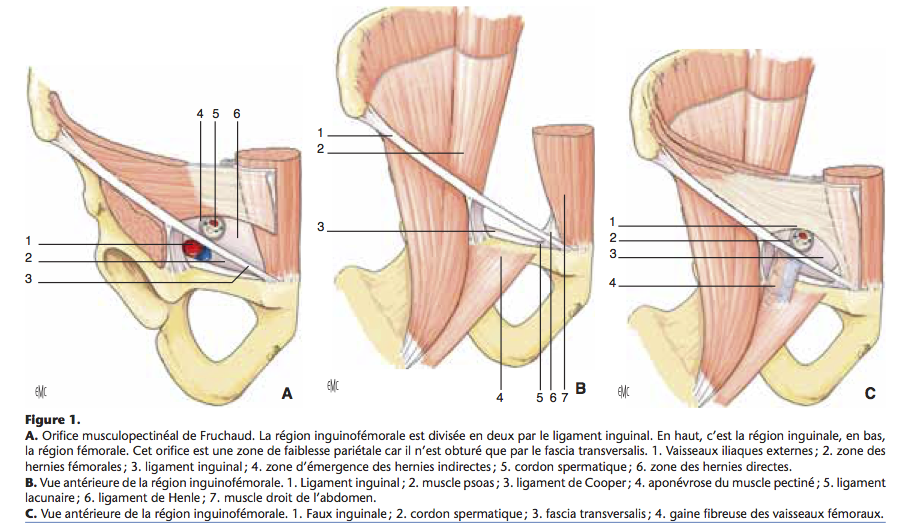
\includegraphics[width=0.70\columnwidth]{figures/Orifice_Pectineal_Fruchaud.png}
\caption{{Orifice pectinéal de Fruchaud
{\label{Orifice_Pectineal}}%
}}
\end{center}
\end{figure}



\begin{figure}[b!]
\begin{center}
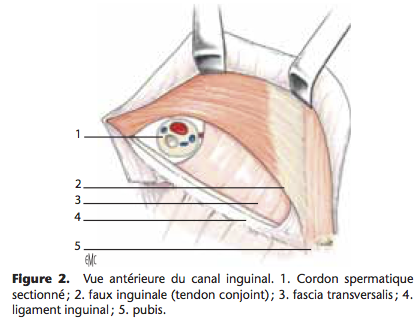
\includegraphics[width=0.70\columnwidth]{figures/Vue_Anterieure_Canal_Inguinal.png}
\caption{{Vue antérieure du canal inguinal.
{\label{Vue_Anterieure}}%
}}
\end{center}
\end{figure}

\begin{figure}[b!]
\begin{center}
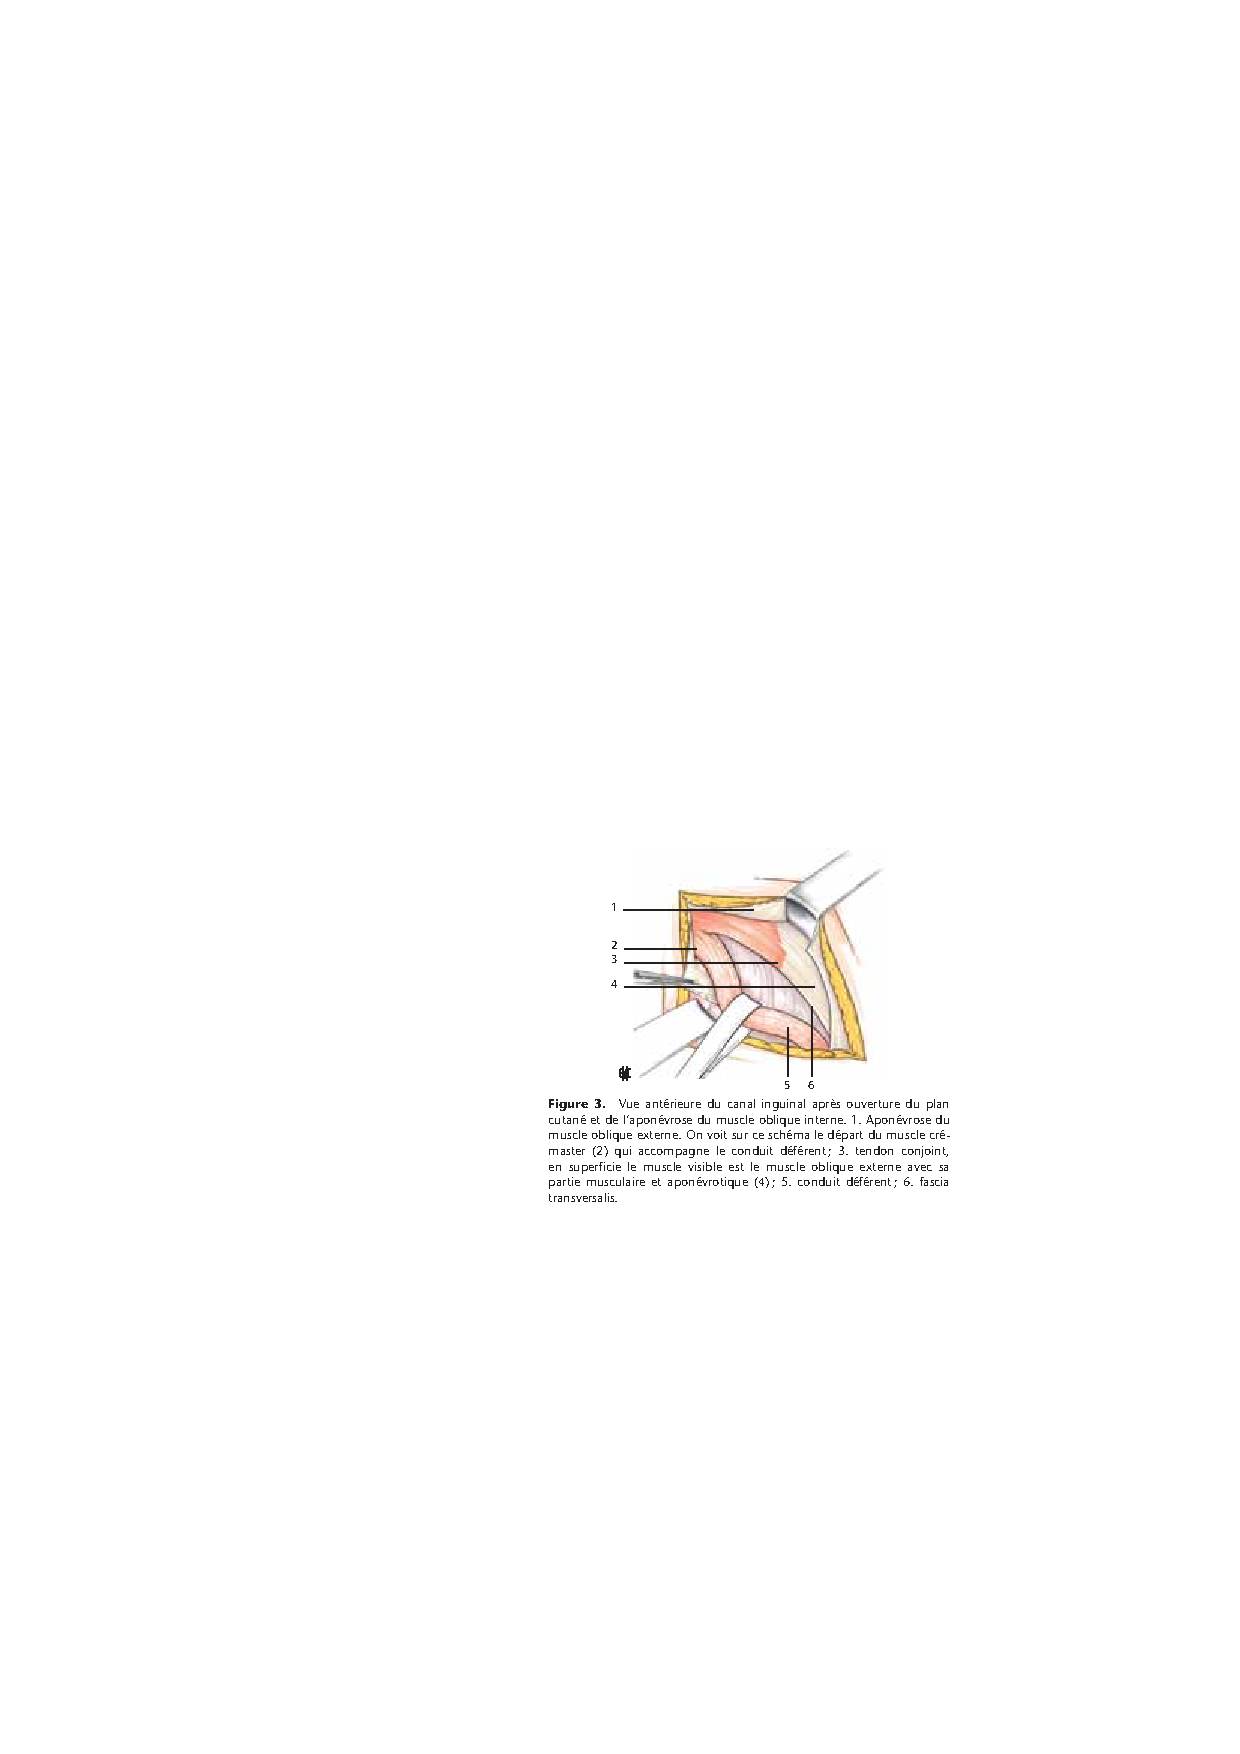
\includegraphics[width=0.70\columnwidth]{figures/Vue_Anterieure_Canal_Inguinal_Apres_Ouverture.pdf}
\caption{{Vue antérieure du canal inguinal après ouverture du plan cutané et de l'aponévrose du muscle interne.
{\label{Vue_Anterieure_Ouverture}}%
}}
\end{center}
\end{figure}

\begin{figure}[b!]
\begin{center}
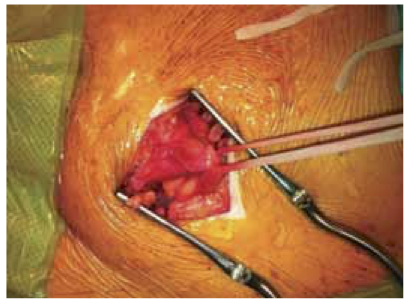
\includegraphics[width=0.70\columnwidth]{figures/Cordon_Testiculaire/Cordon_Testiculaire.png}
\caption{{Cordon testiculaire isolé sur les lacs
{\label{cordon_testiculaire}}%
}}
\end{center}
\end{figure}

\pagebreak

\selectlanguage{french}
\clearpage
\section*{\refname}\sloppy
\phantomsection
\label{csl:1}1. Zhou J, Xue Z, Du Z, Melese T, Boyer PD. {Relationship of tightly bound {ADP} and {ATP} to control and catalysis by chloroplast {ATP} synthase}. Biochemistry [Internet] 1988;27:5129–35. Available from: \url{https://doi.org/10.1021\%2Fbi00414a027}

\phantomsection
\label{csl:2}2. Boyer PD. {Energy Life, and {ATP} (Nobel Lecture)}. Angewandte Chemie International Edition [Internet] 1998;37:2296–307. Available from: \url{https://doi.org/10.1002\%2F\%28sici\%291521-3773\%2819980918\%2937\%3A17\%3C2296\%3A\%3Aaid-anie2296\%3E3.0.co\%3B2-w}

\phantomsection
\label{csl:3}3. Pans A, Albert A, Lapière CM, Nusgens B. {Biochemical study of collagen in adult groin hernias.}. J Surg Res 2001;95:107–13. 

\phantomsection
\label{csl:4}4. Jansen PL, Mertens PP, Klinge U, Schumpelick V. {The biology of hernia formation.}. Surgery 2004;136:1–4. 

\phantomsection
\label{csl:5}5. Rosch R, Klinge U, Si Z, Junge K, Klosterhalfen B, Schumpelick V. {A role for the collagen I/III and MMP-1/-13 genes in primary inguinal hernia?}. BMC Med Genet 2002;3:2. 

\phantomsection
\label{csl:6}6. Lichtenstein IL, Shulman AG, Amid PK, Montllor MM. {The tension-free hernioplasty.}. Am J Surg 1989;157:188–93. 

\end{document}

